\documentclass[tikz]{standalone}
\usepackage{pgfplots}
\pgfplotsset{compat=1.8,
    scale only axis,
    xlabel near ticks,
    ylabel near ticks,
    every axis title shift=3pt}

\usetikzlibrary{arrows.meta}
\usepgfplotslibrary{groupplots}

\begin{document}

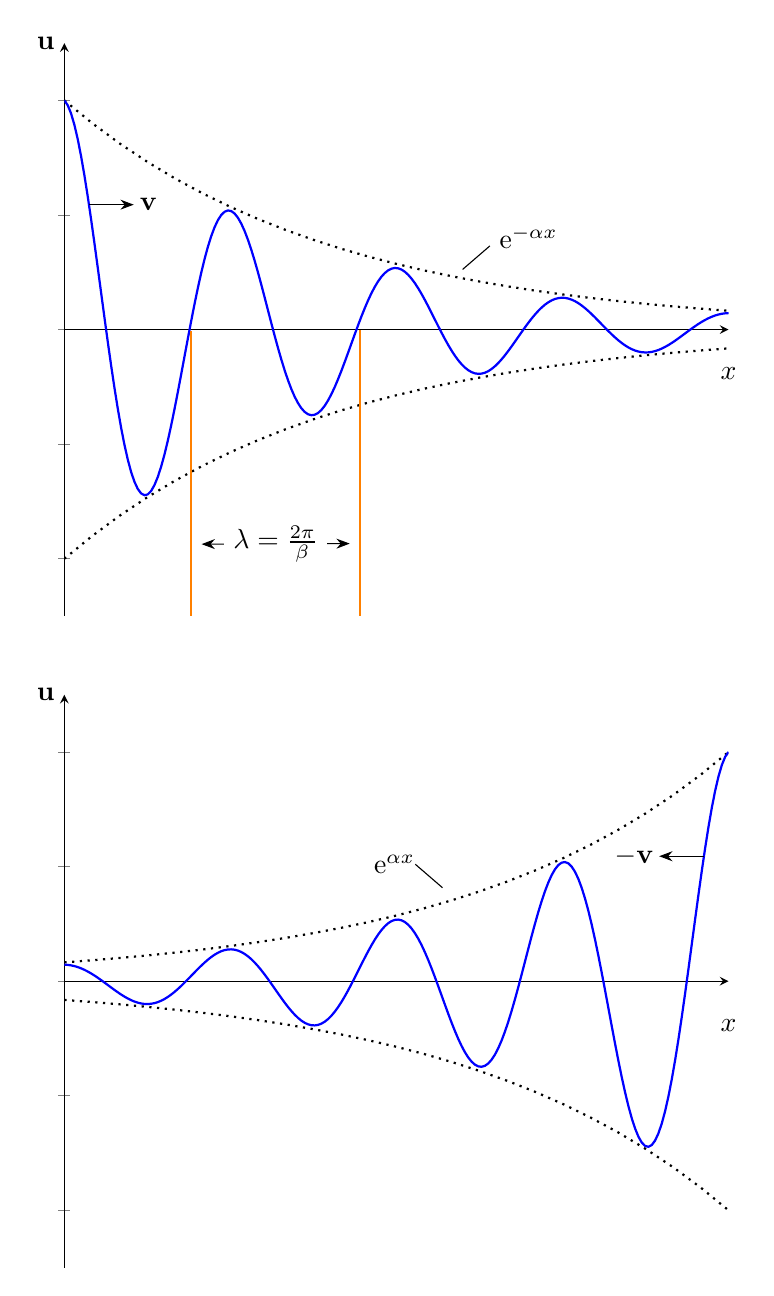
\begin{tikzpicture}

\pgfplotsset{xmin=0, xmax=25, ymin=-1.25, ymax=1.25,
    axis x line=center,
    axis y line=left,
    xlabel=$x$,
    ylabel=$\textbf{u}$,
    ylabel style={rotate=-90, at={(current axis.above origin)}, anchor=east},
    xlabel style={at={(axis description cs:1,0.45)},anchor=north},
    xtick={0},
    yticklabels={},
    % scale y
%    y=1cm
}


\begin{groupplot}[group style={group size=1 by 2,
horizontal sep=1cm,
vertical sep=1cm}]

\nextgroupplot[]

%envelope
\addplot[thick, dotted, domain=0:25] {exp(-0.1*x)} node[pos=0.6, left] (A1) {};
\addplot[thick, dotted, domain=0:25] {-exp(-0.1*x)};

\draw (A1) -- +(45:20) node[right, yshift=3pt] {$\mathrm{e}^{- \alpha x}$};

% cos
\addplot[thick, blue, domain=0:25, samples=200] {exp(-0.105*x) * cos(deg(x))} node[pos=0.04, left] (V1) {}
node[pos=0.21] (N1) {} node[pos=0.465] (N2) {};

\draw[thick, orange] (N1) -- +(-90:4cm) node[pos=0.7] (N121) {};
\draw[thick, orange] (N2) -- +(-90:4cm) node[pos=0.7] (N122) {};
\draw[Stealth-Stealth] (N121) -- (N122) node[pos=0.5, fill=white] {$\lambda = \frac{2 \pi}{\beta}$};

\draw[-Stealth] (V1) -- +(0:0.7cm) node[right, inner sep=2pt] {$\textbf{v}$};



\nextgroupplot[]

%envelope
\addplot[thick, dotted, domain=0:25] {exp(-0.1*(25-x))} node[pos=0.6, left] (A1) {};
\addplot[thick, dotted, domain=0:25] {-exp(-0.1*(25-x))};

\draw (A1) -- +(135:20) node[left, inner sep=0] {$\mathrm{e}^{\alpha x}$};

% cos
\addplot[thick, blue, domain=0:25, samples=200] {exp(-0.105*(25-x)) * cos(deg(25-x))} node[pos=0.96, right] (V1) {};

\draw[-Stealth] (V1) -- +(180:0.7cm) node[left, inner sep=2pt] {$-\textbf{v}$};


\end{groupplot}

\end{tikzpicture}


\end{document}